\documentclass[../ana1.tex]{subfiles}
\onlyinsubfile{\sectionNumbering} %Use numbering relative to sections and not subsection

\begin{document}
\setcounter{section}{17}
\section{Die Ableitung}

Im Folgenden \( I \subset \R \) offenes Intervall, 
\( f: I \rightarrow \R \) (oder \( \C \ko \R^d \)).

\begin{defi}[Ableitung]
    \( f : I \rightarrow \R \) (oder \( \C \ko \R^d \)) 
    hat in \( x_0 \in I \) die Ableitung \( a\in \R \) 
    (oder \( \C \ko \R^d \)), falls 
    \[ \limesx{x}{x_0} \underbrace{\frac{f(x) - f(x_0)}{x - x_0}}_{
        \text{Differenzenquotient}
    } = a. \; (*) \]
    Notation: \( f'(x_0) := a \).\\
    Nennen \(f\) differenzierbar (diffbar) in \(x_0\), falls 
    es so ein \(a\) mit \((*)\) gibt, falls also der Grenzwert 
    in \((*)\) existiert.\\
    Bild:
    \begin{center}
        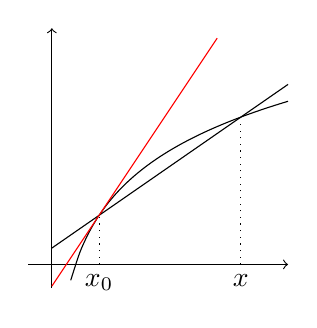
\begin{tikzpicture}[scale = 0.3]
            \draw[->] (0,-1) -- (0,10);
            \draw[->] (-1,0) -- (10,0);
            \draw[thin,domain=0.8:10,smooth,variable=\x,black] plot ({\x},{3 * ln(\x)});
            \draw[thin,domain=0:10,smooth,variable=\x,black] plot ({\x},{0.693 * (\x + 1)});
            \draw[thin,domain=0:7,smooth,variable=\x,red] plot ({\x},{1.5 * \x - 0.921});
            \draw[dotted] (2,0) node[below] {\(x_0\)} -- (2,2.079);
            \draw[dotted] (8,0) node[below] {\(x\)} -- (8,6.238);
        \end{tikzpicture}
    \end{center}
    Sekante: Steigung der Geraden durch \( (x_0, f(x_0)) \) und 
    \((x, f(x)) = \frac{f(x) - f(x_0)}{x - x_0}\).\\
    Tangente mit Steigung \( = f'(x_0) = a \).\\
    Alternativ, \( x = x_0 + h \Rightarrow x - x_0 = h \)
    \[ \limesx{h}{0} \frac{f(x_0 + h) - f(x_0)}{h} = a =: f'(x_0) \]
\end{defi}

\begin{bem}
    Konvergenz bezüglich Euklidischer Norm in \( \R^d 
    \Leftrightarrow \) Konvergenz der Koordinaten.
\end{bem}
\begin{lem}
    Die Funktion \( f : I \rightarrow \R^d \) ist in \(x_0\) 
    differenzierbar \( \Leftrightarrow f = (f_1,f_2,\ldots,f_d) \), 
    alle \( f_j : I \rightarrow \R \) sind in \( x_0 \) 
    differenzierbar.
    \[ \frac{f(x) - f(x_0)}{x-x_0} = \left( 
        \frac{ f_1(x) - f_1(x_0) }{x-x_0} \ko
        \frac{ f_2(x) - f_2(x_0) }{x-x_0} \ko
        \ldots \ko
        \frac{ f_d(x) - f_d(x_0) }{x-x_0} \right) 
        \rightarrow (f_1'(x_0), f_2'(x_0), \ldots, f_d'(x)) \]
\end{lem}
\begin{bsp}
    \( f: I \rightarrow \R^3, f(t) = (x(t), y(t), z(t)) \) 
    Durchschnittsgeschwindigkeit im Intervall \( [t_0, t] 
    \subset I \) ist \( \frac{f(t) - f(t_0)}{t - t_0} 
    \overset{t\rightarrow t_0}{\longrightarrow} \underbrace{ 
        f'(t_0) }_{ = (x'(t), y'(t) ,z'(t))}
    = v(t_0) \) \gqq{instante Geschwindigkeit}.
\end{bsp}
\begin{defi}[Ableitungsfunktion]
    \( f : I \rightarrow \R^d \) (\( \C, \R^d \)) heißt 
    differenzierbar (diffbar) auf \(I\) (einfach differenzierbar), 
    falls \(f\) in jedem Punkt \( x_0 \in I \) differenzierbar ist. \\
    Die hierdurch gegebene Funktion 
    \[ f': I \rightarrow \R^d, x_0 \mapsto f'(x_0) 
    = \limesx{x}{x_0} \frac{f(x) - f(x_0)}{x - x_0} \]
    heißt Ableitungsfunktion oder kurz Ableitung.
\end{defi}
\begin{bspe}\leavevmode
    \begin{enumerate}
        \item 
        Konstante Funktion \( f : I \rightarrow \R^d, f(x) = c, 
        c \in \R^d \) fest.
        \[ x \neq x_0 \Rightarrow \frac{f(x) - f(x_0)}{x-x_0} 
        = \frac{c - c}{x - x_0} = 0 \Rightarrow f'(x_0) = 0 
        \,\forall \, x_0 \in I. \]
        \item 
        \( f: \R \rightarrow \R, x \mapsto f(x) = x \). \\
        \[ \frac{f(x) - f(x_0)}{ x-x_0 } 
        = \frac{x - x_0}{x - x_0} = 1 \Rightarrow f'(x_0) = 1. \]
        \item 
        \( f : \R \rightarrow \R, x \mapsto f(x) = \abs{x} \)
        ist nicht in \(0\) differenzierbar. 
        \begin{center}
            \begin{tikzpicture}[scale = 3]
                \draw[->] (0,-0.1) -- (0,1) node[above] {\(f(x)\)};
                \draw[->] (-1,0) -- (1,0) node[right] {\(x\)};
                \draw[thin,domain=-0.75:0.75,smooth,variable=\x,black] plot ({\x},{abs(\x)});
            \end{tikzpicture}
        \end{center}
        \[ \limesx{x}{0+} \frac{f(x) - f(0)}{x - 0} 
        = \limesx{x}{0+} \frac{x}{x} = 1 \]
        \[ \limesx{x}{0-} \frac{f(x) - f(0)}{x - 0} 
        = \limesx{x}{0-} \frac{\abs{x}}{x} 
        = \limesx{x}{0-} \frac{-x}{x} = \minus 1. \]
        \item 
        \( n\in\N, f: \R \rightarrow \R, x \mapsto x^n \).
        \begin{align*}
            x^n - x_0^n &= (x-x_0)( x^{n-1} + x^{n-2}x_0 
            + x^{n-3}x_0^2 + \cdots + x x_0^{n-2} + x_0^{n-1} )\\
            &= (x - x_0) \sum_{j=0}^{n-1} (x^{n-j-1} x_0^j) \\
            &= \sum_{j=0}^{n-1} x x^{n-1-j} x_0^j 
            - \sum_{j=0}^{n-1} x^{n-1-j} x_0^{j+1} \qquad l := j+1\\
            &= \sum_{j=0}^{n-1} x^{n-j} x_0^j - \sum_{l=1}^n x^{n-l} x_0^l \\
            &= x^n - x_0^n \; \checkmark
        \end{align*}
        \begin{align*}
            &\Rightarrow \frac{x^n - x_0^n}{ x - x_0 } \\
            &= \frac{ (x - x_0) \sum_{j=0}^{n-1} x^{n-1-j}x_0^j }{x-x_0} \\
            &= \sum_{j=0}^{n-1} x^{n-1-j} x_0^j \overset{
                x \rightarrow x_0}{\longrightarrow
            } \sum_{j=0} ^{n-1} x_0^{n-1-j} x_0^j \\
            &= n x_0^{n-1}.
        \end{align*}
        D.\ h.\  \( f_n(x) = x^n \) ist differenzierbar. 
        \( f'(x) = n x^{n-1} \).
    \end{enumerate}
\end{bspe}
\begin{satz}[differenzierbar \( \Rightarrow \) stetig]
    \( I \) offenes Intervall \( f : I \rightarrow \R^d \) 
    differenzierbar in \( x_0 \in I \Rightarrow f \) ist stetig 
    in \(x_0\).
\end{satz}
\begin{bew}
    Sei \( x\in I, x \neq x_0 \).
    \[ f(x) = f(x_0) + \underbrace{
    \frac{f(x) - f(x_0)}{x - x_0} }_{
        \underset{x\rightarrow x_0}{\longrightarrow} f'(x_0)
    } \underbrace{(x-x_0)}_{\rightarrow 0} 
    \overset{x\rightarrow x_0 }{\longrightarrow} 
    f(x_0) + f'(x_0) \cdot 0 = f(x_0). \]
    \( \Rightarrow \limesx{x}{x_0} f(x) = f(x_0) \), also ist
    \( f \) stetig in \( x_0 \).
\end{bew}
\begin{satz}[Differentiationsregeln]\label{satz:diff_regeln}
    Seien \( f, g: I \rightarrow \R^d \) differenzierbar in \(x_0\)
    \[ \Rightarrow \alpha f + \beta g, \alpha, \beta \in \R 
    \text{ ist in } x_0 \text{ differenzierbar.} \]
    und 
    \begin{enumerate}
        \item Linearität 
        \[ (\alpha f + \beta g)'(x_0) = \alpha f'(x_0) 
        + \beta g'(x_0) \]
        (ähnlich: \( f, g: I \rightarrow \C, \alpha, \beta \in \C \).)
    \end{enumerate}
    Sind \( f, g: I \rightarrow \R \) (oder \( \C \)) in \(x_0\)
    differenzierbar, so sind auch \( f\cdot g \) und im Fall 
    \( g(x_0) \neq 0 \) \( \frac{f}{g} \) differenzierbar und 
    \begin{enumerate}
        \setcounter{enumi}{1}
        \item Produktregel
        \[ (f \cdot g)'(x_0) = f'(x_0) \cdot g(x_0) 
        + f(x_0) \cdot g'(x_0) \]
        \item Quotientenregel
        \[ \left( \frac{f}{g} \right)'(x_0) 
        = \frac{ f'(x_0) g(x_0) - f(x_0) g'(x_0) }{ {g(x_0)}^2 }. \]
        \[ \left(\frac{Z}{N}\right)' = \frac{NAZ - ZAN}{N^2} \]
        \( NAZ = \) Nenner mal Ableitung Zähler\\
        \( ZAN = \) Zähler mal Ableitung Nenner.
    \end{enumerate}
\end{satz}
\begin{bew}
    \begin{enumerate}
        \item 
        \begin{align*}
            &\frac{ (\alpha f + \beta g)(x) 
            - (\alpha f + \beta g)(x_0) }{ x - x_0 } \\
            &= \alpha \frac{ f(x) - f(x_0) }{x - x_0} + 
            \beta \frac{ g(x) - g(x_0) }{x - x_0}\\
            &\rightarrow \alpha f'(x_0) + g'(x_0).
        \end{align*}
        \item 
        \begin{align*}
            &\frac{ f(x) g(x) - f(x_0)g(x_0) }{ x - x_0 }\\ 
            &= \frac{ (f(x) - f(x_0))g(x) + f(x_0)g(x) 
            - f(x_0)g(x_0) }{ x - x_0 }\\
            &= \underbrace{\frac{f(x) - f(x_0)}{ x - x_0 }}_{
                \rightarrow f'(x_0)} \underbrace{g(x)}_{
                    \substack{=g(x_0),\\ \text{da auch}\\ \text{stetig in } x_0}} 
            + f(x_0) \underbrace{\frac{g(x) - g(x_0)}{ x - x_0 }}_{
                \rightarrow g'(x_0)} \\
            &\overset{x\rightarrow x_0}{\longrightarrow} f'(x_0) g(x_0) + f(x_0) g'(x_0)
        \end{align*}
        \item
        Erstmal \( f(x) = 1 \,\forall \, x \in I \).
        \[ \frac{1}{g(x)} - \frac{1}{g(x_0)} 
        = \frac{g(x_0) - g(x)}{g(x) g(x_0)} \]
        \[ \Rightarrow \frac{1}{x - x_0} 
        \left( \frac{1}{g(x)} - \frac{1}{g(x_0)} \right)
        = - \frac{1}{g(x) g(x_0)} \cdot \frac{g(x) - g(x_0)}{x - x_0} 
        \overset{x\rightarrow x_0}{\longrightarrow} 
        - \frac{g'(x_0)}{{g(x_0)}^2} \]
        Allgemein \(f\): schreibbar \( \frac{f}{g} = f \cdot \frac{1}{g} \) 
        und Produktregel.
    \end{enumerate}
\end{bew}
\begin{bsp}\leavevmode
    \begin{enumerate}
        \setcounter{enumi}{4}
        \item Sei \( f_n : \R \rightarrow \R, f_n(x) = x^n, n\in\N \)
        \( \overset{\text{Bsp.\ 2}}{\Rightarrow} f_1'(x) = 1 \)
        \begin{align*}
            \overunderset{\hyperref[satz:diff_regeln]{\text{Produkt-}}}{
                \hyperref[satz:diff_regeln]{\text{regel}}}{\Rightarrow} 
            f_n'(x) &= (f_1 \cdot f_{n-1})'(x) \\
            &= f_1'(x) f_{n-1}(x) + f_1(x) f_{n-1}'(x)\\
            &= f_{n-1}(x) + x f_{n-1}'(x) = x^{n-1} + x f_{n-1}'(x)
        \end{align*}
        \begin{align*}
            n=2: & f_2'(x) = x + x \cdot 1 = 2x\\
            n=3: & f_3'(x) = x^2 + x f_2(x) = x^2 + x 2x = 3x^2
        \end{align*}
        Weiter per Induktion: \( f_n'(x) = n x^{n-1} \)
        Allgemein folgt aus Satz 5 (1) für Polynome
        \begin{align*}
            p(x) &= \sum_{k=0}^n a_k x^k \\
            p'(x) &= \sum_{k=1}^n a_k \cdot k \cdot x^{k-1} 
            = \sum_{k=0}^{n-1} (k + 1)a_{k+1} \cdot x^k
        \end{align*}
        \item
        \( f_n: \R \setminus \set{0} \rightarrow \R, 
        x \mapsto x^{-n} = \frac{1}{x^n} \, n\in\N \) fest.
        \[ \overunderset{\text{Quotienten-}}{\text{regel}}{\Rightarrow} 
        f_n'(x) = \left( \frac{1}{x_n} \right)' 
        = \frac{-n x^{n-1}}{{(x^n)}^2} \]
    \end{enumerate}
\end{bsp}
\begin{satz}[Kettenregel]
    Seien \( f: I \rightarrow \R, g : J \rightarrow \R, f(I) \subset J \). 
    Ist \( f \) in \( x_0 \in I \) differenzierbar und \(g\) in 
    \( y_0 := f(x_0) \) differenzierbar, so ist auch 
    \( g \circ f : I \rightarrow \R, (g \circ f)(x) = g(f(x)) \) in \(x_0\) 
    differenzierbar und 
    \[ (g \circ f)'(x_0) = g'(f(x_0)) \cdot f'(x_0) \]
\end{satz}
\begin{bew}
    Sei \( x \neq x_0 \).
    \[ \frac{ g(f(x_0)) - g(f(x_0)) }{ x - x_0 } = \begin{cases}
        \frac{ g(f(x)) - g(f(x_0)) }{f(x) - f(x_0)} 
        \frac{ f(x) - f(x_0) }{ x-x_0 }, &\text{falls } f(x) \neq f(x_0)\\
        0, &\text{falls } f(x) = f(x_0)
    \end{cases} \]
    Definiere \[ \tilde{g} : J \rightarrow \R, \tilde{g}(y) := \begin{cases}
        \frac{ g(y) - g(y_0) }{ y - y_0 }, &y \neq y_0\\
        g'(y_0), &y=y_0
    \end{cases} \]
    \( y_0 := f(x_0) \).
    \[ \Rightarrow \limesx{y}{y_0} \tilde{g}(y) = g'(y_0) = \tilde{g}(y_0). \]
    Somit ist \( \tilde{g} \) in \(y_0\) stetig.
    \[ \Rightarrow \frac{ g(f(x)) - g(f(x_0)) }{ x - x_0 } 
    = \tilde{g}(f(x)) \frac{ f(x) - f(x_0) }{x - x_0}. \]
    \begin{align*}
        &\Rightarrow \limesx{x}{x_0} \frac{ g(f(x)) - g(f(x_0)) }{ x - x_0 } \\
        &= \limesx{x}{x_0} \left( \tilde{g}(f(x)) \frac{f(x) - f(x_0)}{x - x_0} \right) \\
        &= \limesx{x}{x_0} \tilde{g}(f(x)) \limesx{x}{x_0} \frac{f(x) - f(x_0)}{x - x_0} \\
        &= \tilde{g}(f(x_0))f'(x_0) = g'(f(x_0)) f'(x_0).
    \end{align*}
\end{bew}
Ang.: \( f : I \rightarrow J\) bijektiv, \( I, J \) offene Intervalle und 
\( g = \inverse{f} : J \rightarrow I \).\\
Ang.: \( g \) ist differenzierbar in \( y_0 \in J, y_0 = f(x_0) \) und 
\( f \) ist differenzierbar in \(x_0\).
\[\forall \, x\in I: x = g(f(x)) \overset{\text{Ableiten}}{\Rightarrow} 1 = (g(f(x_0)))' 
= g'(f(x_0)) \cdot f'(x_0) \]
\[ \Rightarrow f'(x_0) \neq 0 \text{ und } y_0 = f(x_0) \]
\[ g'(y_0) = \frac{1}{f'(x_0)} = \frac{1}{f'(g(y_0))} 
\Leftrightarrow g'(f(x_0)) = \frac{1}{f'(x_0)}. \]
\begin{satz}[Differenzierbarkeit der Umkehrfunktion]\label{satz:diffbar_umkehr}
    Sei \( f: I \rightarrow \R \) streng wachsend und stetig auf 
    dem Intervall \(I\) mit Endpunkten \( a < b \). Dann gilt 
    \begin{enumerate}
        \item \( J = f(I) \) ist ein Intervall mit Endpunkten 
        \[ \alpha := \limesx{x}{a +} f(x) 
        < \beta := \limesx{x}{b -} f(x) \]
        \item Die Umkehrfunktion \( g: J = f(I) \rightarrow I \) ist 
        ebenfalls stetig und streng wachsend.
        \item \( \limesx{y}{\alpha +} g(y) = a, 
        \limesx{y}{\beta -} g(y) = b \) (Man male ein Bild.)
    \end{enumerate}
    Zudem ist \( I \) ein offenes Intervall, so ist auch \( J = f(I) \) 
    ein offenes Intervall und ist \(f\) in \(x_0\) differenzierbar mit 
    \( f'(x) \neq 0 \), so ist \(g\) differenzierbar in \( y_0 = f(x_0) \) 
    mit 
    \[ g'(y_0) = \frac{1}{f'(g(y_0))} = \frac{1}{f'(x_0)}. \]
\end{satz}
\begin{prosa}
    Zum Beweis benötigen wir 
\end{prosa}
\begin{lem}\label{satz:monoton_grenzwert}
    Sei \( h: I \rightarrow \R \) monoton wachsend, \(I\) ein Intervall mit 
    Endpunkten \( a < b \).\\
    Dann hat \(h\) einseitige Grenzwerte. Genauer
    \[ \limesx{x}{x_0 -} h(x) = \lim\limits_{x \nearrow x_0} h(x) 
    = \sup \underset{\text{falls } x_0 > a}{\set{ h(x) 
    \; \vert \; x \in I, x < x_0 }} \]
    \[ \limesx{x}{x_0 +} h(x) = \lim\limits_{x \searrow x_0} h(x) 
    = \inf \underset{\text{falls } x_0 < b}{\set{ h(x) 
    \; \vert \; x \in I, x > x_0 }} \]
    Analoge Aussage gilt, falls \(h\) monoton fallend ist.
\end{lem}
\begin{bew}[von \autoref{satz:diffbar_umkehr}]
    Schritt 1: \(f\) strikt wachsend. 
    \( \Rightarrow f \) ist injektiv \( \Rightarrow f : 
    I \rightarrow f(I) \) ist injektiv \( \Rightarrow \inverse{f} : 
    f(I) \rightarrow I \) existiert.\\
    Schritt 2: \( J := f(I) \) ist auch Intervall.\\
    Seien \( y_1 < y_2 < J \) und \( y_1 < c < y_2 \)
    \[ \Rightarrow \exists \, x_1 < x_2 \in I : y_1 = f(x_1), 
    y_2 = f(x_2). \]
    \[ f \text{ stetig } 
    \overunderref{satz:zwischenwert}{Zwischen-}{wertsatz}{\Rightarrow}
    \exists \, x_1 < x < x_2: f(x) = c. \]
    \[ \Rightarrow c \in J = f(I). \]
    \[ \Rightarrow [y_1, y_2] \subset J = f(I). \]
    \[ J \text{ ist ein Intervall.} \]
    \[ \oversett{Lemma 8}{\Rightarrow} \exists \, \alpha := 
    \limesx{x}{\alpha +} f(x) < \beta = \limesx{x}{b -} f(x) \]
    \( \alpha \) und \( \beta \) sind Endpunkte von \(J\).\\ 
    \( \Rightarrow \) 1.\ ist gezeigt.\\
    Schritt 3: \\
    \( g: J \rightarrow I \) ist streng wachsend.\\
    Wenn nicht, dann gäbe es 
    \[ y_1 < y_2 \in J : g(y_1) \geq g(y_2) \]
    \[ \Rightarrow y_1 = f(g(y_1)) \geq f(g(y_2)) \text{ \Lightning{}} \]
    Schritt 4: \( g: J \rightarrow I \) ist stetig.\\
    Es reicht zu zeigen: die eindeutigen Grenzwerte sind gleich dem 
    Funktionswert.\\
    \Obda: linksseitiger Grenzwert.
    \[ y_0 = f(x_0) \in (\alpha, \beta] \]
    \[ x_{\minus} := \limesx{y}{y_0 \minus} g(y) 
    = \lim\limits_{y \nearrow y_0} g(y)
    \overset{\text{Ann.}}{<} g(y_0) = x_0. \]
    Bild:
    \begin{center}
        \begin{tikzpicture}[scale = 0.3]
            \draw[->] (0,-1) -- (0,10);
            \draw[->] (-1,0) -- (10,0);
            \draw[thin,domain=2:5,smooth,variable=\x,black] plot ({\x},{3 * ln(\x)});
            \draw[thin,domain=5:8,smooth,variable=\x,black] plot ({\x},{3 * ln(\x) + 1.5}) node[above] {\(g\)};
            \draw (2,0) node {\([\)} node[below=2mm] {\(\alpha \)};
            \draw (8,0) node {\(]\)} node[below=2mm] {\( \beta \)};
            \draw (5,0.5) -- (5,-0.5) node[below] {\(y_0\)};
            \draw (0.5,2) -- (-0.5,2) node[left] {\(a\)};
            \draw (0.5,7.74) -- (-0.5,7.74) node[left] {\(b\)};
            \draw (0.5,6.33) -- (-0.5,6.33) node[left] {\(x_0\)};
            \draw (0.5,4.83) -- (-0.5,4.83) node[left] {\(x_{\minus}\)};
        \end{tikzpicture}
        \begin{tikzpicture}[scale = 0.3]
            \draw[->] (0,-1) -- (0,10);
            \draw[->] (-1,0) -- (10,0);
            \draw[thin,domain=2:5,smooth,variable=\x,black] plot ({ 3 * ln(\x) },{\x});
            \draw[thin,domain=4.83:6.33,smooth,variable=\x,black] plot ({\x},{5});
            \draw[thin,domain=5:8,smooth,variable=\x,black] plot ({ 3 * ln(\x) + 1.5 },{\x}) node[above] {\(f\)};
            \draw (2,0) node {\([\)} node[below=2mm] {\(a\)};
            \draw (8,0) node {\(]\)} node[below=2mm] {\(b\)};
            \draw (0.5,5) -- (-0.5,5) node[left] {\(y_0\)};
            \draw (0.5,2) -- (-0.5,2) node[left] {\( \alpha \)};
            \draw (0.5,7.74) -- (-0.5,7.74) node[left] {\( \beta \)};
            \draw (6.33,0.5) -- (6.33,-.5) node[below] {\(x_0\)};
            \draw (4.83,0.5) -- (4.83,-.5) node[below] {\(x_{\minus}\)};
        \end{tikzpicture}
    \end{center}
    \( g \) streng wachsend \( \Rightarrow a < x < x_0 \) \\
    \( f \) stetig in \(x_0\): 
    \begin{align*}
        &f(x_{\minus})\\
        &= f(\limesx{y}{y_0 \minus} g(y))\\
        &= \limesx{y}{y_0 \minus} f(g(y))\\
        &= \limesx{y}{y_0 \minus} y = y_0\\
        &= f(x_0)
    \end{align*}
    \Lightning{} zu \(f\) streng wachsend.
    Genauso \( \lim \) rechtsseitiger Grenzwert.\\
    Schritt 5: 3.\ folgt durch Anwenden von 
    1.\ und 2.\ auf \(g\) anstatt \(f\).\\
    Schritt 6: Es gilt immer
    \begin{align*}
        &a\in I \Leftrightarrow \alpha \in J = f(I)\\
        \text{und } &b\in I \Leftrightarrow \beta \in J.
    \end{align*}
    Insbesondere \(I\) offen \( \Leftrightarrow J \) offen.\\
    Dann ist \( a \in I \subset [a,b] \)
    \[ \Rightarrow \alpha = \inf \set{ f(x) \;\vert \; x \in I } 
    = f(a) \in f(I) = J. \]
    Umgekehrt: Ist \( \alpha \in J \), so ist 
    \[ a = \inf \set{ g(y) \;\vert \; y \in J } 
    = g(\alpha) \in g(J) = I. \]
    Genauso zeigt man \( b\in I \Leftrightarrow \beta \in J \).\\
    Schritt 7: nach Schritt 6 ist \( J = f(I) \) offenes Intervall, 
    falls \( I \) offenes Intervall und \( g = \inverse{f} \) ist streng 
    wachsend und stetig. Nehme \( y \neq y_0, y, y_0 \in J \).
    \[ \Rightarrow g(y) \neq g(y_0) \]
    \[ \text{und } x = g(y) \rightarrow g(y_0) 
    = x_0 \text{ für } y \rightarrow y_0. \]
    \begin{align*}
        &\frac{ g(y) - g(y_0) }{ y - y_0 }\\
        &= \frac{ g(y) - g(y_0) }{ f(g(y)) - f(g(y_0)) }\\
        &= \frac{1}{ \frac{f(g(y)) - f(g(y_0))}{  g(y) - g(y_0)} }\\
        &= \frac{1}{ \frac{ f(x) - f(x_0) }{ x - x_0 } }
    \end{align*}
    \[ x = g(y), x_0 = g(y_0). \]
    \[ y \rightarrow y_0 \Rightarrow x = g(y) \rightarrow g(y_0) = x_0 \]
    \begin{align*}
        &\limesx{y}{y_{\minus}} \frac{ g(y) - g(y_0) }{ y - y_0 }\\
        &= \limesx{x}{x_0} \frac{1}{ \frac{ f(x) - f(x_0) }{ x - x_0 } }\\
        &= \frac{1}{f'(x_0)} \text{ existiert, da } f'(x_0) \neq 0.
    \end{align*}
    \[ \Rightarrow g'(y_0) = \frac{1}{ f'(x_0) } = \frac{1}{ f'(g(y_0)) }. \]
\end{bew}
\begin{bsp}
    \( f: \R \rightarrow \R, x \mapsto x^3 = f(x) \)
    \[ f'(x) = 3 x^2, f'(0) = 0. \]
    \[ x^3 = y \quad y > 0 \Rightarrow x = y^\frac{1}{3} \]
    Inverse: 
    \[ g(y) = \inverse{f}(y) = \begin{cases}
        y^\frac{1}{3}, &y \geq 0\\
        -{(-y)}^{\frac{1}{3}}, &y \geq 0.
    \end{cases} \]

    \begin{center}
    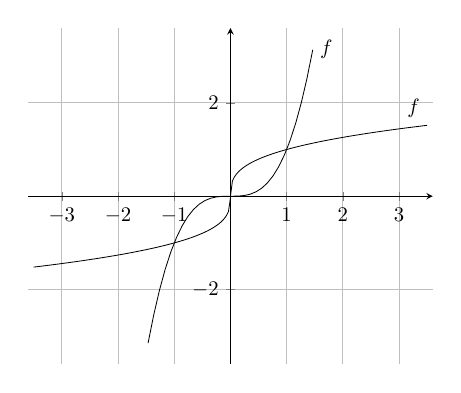
\begin{tikzpicture}[scale=3/4]
        \begin{axis}[grid=both,
            xmin=-3,ymin=-3,
            xmax=3,ymax=3,
            axis lines=middle,
            restrict y to domain=-3.5:3.5,
            restrict x to domain=-4:4,
            enlargelimits]
        \addplot[black,samples=100] {x^3} node[right]{\(f\)};
        \addplot[black,domain=0:3.5,samples=100] {pow(x,1/3)} node[above left] {\( \inverse{f} \)};
        \addplot[black,domain=-3.5:0,samples=100] {-pow(-x,1/3)};
        \end{axis}
    \end{tikzpicture}
    \end{center}
    \[ \frac{ g(y) - g(0) }{ y - 0 } 
    = \abs{y}^{\minus \frac{2}{3}} \rightarrow \infty 
    \text{ für } y \rightarrow 0. \]
\end{bsp}
\begin{bew}[von \autoref{satz:monoton_grenzwert}]
    Sei \( x_0 > \alpha \).\\
    \( h : I \rightarrow \R \) monoton wachsend. 
    \( I \) hat Endpunkte \( a < b \).\\
    Sei \( x_0 > a \). 
    \[ \gamma := \sup \set{ h(x) \;\vert \; x \in I, x < x_0 } \]
    \[ \Rightarrow \forall \, \tilde{\gamma} < \gamma 
    \,\exists \, x' \in I, x' < x_0 : h(x') > \tilde{\gamma}. \]
    \( h \) ist monoton wachsend 
    \[ \Rightarrow \tilde{\gamma} < h(x') \leq h(x) \leq \gamma 
    \;\forall \, x' \leq x < x_0 \]
    \[ \Rightarrow \limesx{x}{x_0 \minus} h(x) \text{ existiert.} \]
    \[ \text{und } h(x) = \gamma 
    = \sup \set{ h(x) \;\vert \; x \in I, x < x_0 }. \]
    Zweite Behauptung analog.
\end{bew}
\begin{bem}
    \[ f'(x_0) = \limesx{x}{x_0} \frac{f(x) - f(x_0)}{ x - x_0 } \]
    \[ \Leftrightarrow \limesx{x}{x_0} \underbrace{ \frac{1}{x - x_0} \left(
        f(x) - \set{ f(x_0) + f'(x_0)(x-x_0) } \right) 
    }_{=\varepsilon(x)} = 0 \]
    \( x \neq x_0, \varepsilon(x_0) := 0 \).\\
    D.\ h.\  \( \exists \, \text{ Funktion } 
    \varepsilon : I \rightarrow \R, \varepsilon (x_0) = 0, \varepsilon \) 
    ist stetig in \(x_0\).
    \[ f(x) = \underbrace{f(x_0) + f'(x_0)(x - x_0)}_{
        \text{affin linear}
    } + \underbrace{\varepsilon(x)(x - x_0)}_{\substack{
        \text{Fehler, geht schneller}\\\text{als linear gegen Null}\\
        x \rightarrow x_0}} \]
    Bild:
    \begin{center}
        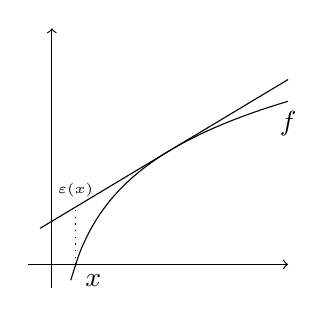
\begin{tikzpicture}[scale = 0.3]
            \draw[->] (0,-1) -- (0,10);
            \draw[->] (-1,0) -- (10,0);
            \draw[thin,domain=0.8:10,smooth,variable=\x,black] plot ({\x},{3 * ln(\x)}) node[below] {\(f\)};
            \draw[thin,domain=-0.5:10,smooth,variable=\x,black] plot ({\x},{0.6 * \x + 1.828});
            \draw[dotted] (1,0) -- (1,2.428) node[above] {\tiny\( \varepsilon(x) \)};
            \draw (1,0) node[below right] {\(x\)};
        \end{tikzpicture}
    \end{center}
\end{bem}
\end{document}